% Final
\section{Návrh vzhledu uživatelského rozhraní}

% Final
V této sekci se zaměřím na samotný vzhled uživatelského rozhraní, konkrétně na volbu barev, písma, ikon a vhodných animací. Cílem je vytvořit konzistentní vzhled, který bude následně možné použít v návrhu uživatelského rozhraní a následně v samotné aplikaci.

% Final
Jelikož stávající aplikace využívá knihovnu Material UI, která implementuje standard Material Design 2 \cite{MaterialUI}, budu celý návrh zakládat na tomto standardu. Zmíněný standard klade důraz na konzistentní využívání palety barev, typografické hierarchie a jednotlivých komponentů. Dále se také zaměřuje na přístupnost uživatelského rozhraní, podporu světlého i tmavého režimu a dodržování osvědčených postupů při návrhu uživatelského rozhraní \cite{MaterialDesign2}.

% Final
Na tomto místě je vhodné zmínit, že v současné době již existuje nová verze tohoto standardu Material Design 3\footnote{Dostupné na: \href{https://m3.material.io/}{https://m3.material.io/}}, nicméně v době psaní tohoto textu nejsou k dispozici žádné knihovny, které by tento standard implementovaly v takové míře, aby je bylo možné pro tento projekt vhodně využít. Proto budu nadále pro aplikaci využívat knihovnu Material UI, která se řídí standardem Material Design 2.

% Final
\subsection{Zásady návrhu}

% Final
Před samotnou tvorbou návrhu je třeba stanovit základní zásady, kterými se bude nový vzhled uživatelského rozhraní řídit. Při sestavování těchto zásad budu vycházet z několika zdrojů. Zaprvé budu vycházet z analýzy existujících aplikací, které jsem se věnoval v předchozí kapitole.

% Final
Zadruhé budu vycházet z toho, jakým způsobem by měla aplikace působit na cílové uživatele. Aplikace by například měla působit jako důvěryhodný zdroj informací, aby ji uživatel vnímal jako vhodný nástroj pro své vzdělávání.

% Final
Zatřetí jsem se rozhodl zaměřit na návrh s ohledem na emoční potřeby uživatelů \cite[385]{Hartson2019TheUxBook}. Emoční potřeby uživatelů mohou být při návrhu určitých typů systémů klíčové a mohou aplikaci zásadně odlišit od konkurenčních řešení \cite[387]{Hartson2019TheUxBook}. Pokud například navrhujeme aplikaci pro děti, můžeme se cíleně zaměřit na návrh uživatelského rozhraní, které bude barevné, interaktivní a zábavné na používání. U jiných typů systémů, jako například v aplikaci obchodní burzy, by podobný způsob designu pravděpodobně působil dětinsky, neprofesionálně a nedůvěryhodně. Jelikož se v rámci této práce zaměřuji na tvorbu vzdělávací aplikace, mohou být motivace a pocity pokroku a úspěchu klíčové, a proto se na ně také zaměřím při návrhu uživatelského rozhraní.

% Final
Na základě zmíněných zdrojů jsem tak identifikoval následující zásady, kterými se budu při návrhu řídit.

% Final
\paragraph{Minimalismus} Hlavním zaměřením aplikace je učit uživatele programování. Při takové činnosti je po uživateli vyžadována vysoká úroveň pozornosti a koncentrace. Ve srovnání s ostatními aplikacemi tak může být používání této aplikace značně kognitivně náročné. Proto jsem se rozhodl při návrhu zaměřit na minimalistický design. Design by tak měl co nejvíce omezit zbytečné informace a zjednodušit prvky uživatelského rozhraní tak, aby nepřehlcovaly uživatele a neodváděly jeho pozornost od učení a dalších klíčových funkcí. Uživatelské rozhraní by tak mělo svým minimalismem pomoci uživateli při učení a používání aplikace.

% Final
\paragraph{Důvěryhodnost} Jelikož se aplikace zaměřuje na výuku a předávání informací uživatelům, je naprosto klíčové, aby působila jako důvěryhodný zdroj informací. Uživatelské rozhraní by tak mělo působit moderně, důvěryhodně a profesionálně.

% Final
\paragraph{Zábava} Jedním z cílů návrhu je motivovat uživatele k dlouhodobému učení a používání aplikace. Proto by pro uživatele mělo být učení a používání aplikace zábavné a měl by se chtít k aplikaci dlouhodobě vracet.

% Final
\paragraph{Pokrok a úspěch} Při používání aplikace, zejména při učení, by měl mít uživatel pocit, že dělá pravidelně pokrok a že se posouvá blíže ke svému cíli. Aplikace by tak měla uživateli často připomínat a zobrazovat jeho pokroky a úspěchy.

% Final
V následujících sekcích na základě těchto zásad vyberu konkrétní barvy, písma, ikony a animace.

% Final
\subsection{Výběr palety barev}

% Final
Jako první krok návrhu vzhledu jsem se rozhodl zvolit paletu barev\footnote{Dostupné na: \href{https://www.figma.com/design/VZFuqWojrXq8yWjrBIq4OH}{https://www.figma.com/design/VZFuqWojrXq8yWjrBIq4OH}}. Vybrané barvy pak budu konzistentně využívat napříč prototypem a celou aplikací. Barvy budu volit v souladu se standardem Material Design 2 a budu volit barvy jak pro světlý, tak pro tmavý režim uživatelského rozhraní. Při volbě palety barev se také budu řídit standardem přístupnosti \textit{Web Content Accessibility Guidelines 2.2} \cite{WCAG22}, díky kterému by mělo být uživatelské rozhraní dobře použitelné napříč různými zařízeními a také použitelné osobami se zdravotním postižením, jako například osobami se sníženým barvocitem.

% Final
\subsubsection{Primární barva}

% Final
Jako první se zaměřím na volbu primární barvy. Tato barva reprezentuje samotnou značku aplikace a je napříč aplikací nejčastěji používána \cite{MaterialDesignColorSystem}. Využívá se zejména ke zvýraznění důležitých prvků, kterými jsou například tlačítka nebo navigační lišty.

% Final
Barvu jsem se rozhodl zvolit v souladu se stanovenými zásadami tak, aby aplikace působila důvěryhodně a profesionálně. Proto jsem jako primární barvu zvolil odstín modré, protože tato barva bývá považována za barvu důvěryhodnosti, inteligence a přesnosti \cite{NURColors}.

% Final
Jako základ pro volbu primární barvy jsem vybral světle modrou s kódem \texttt{\#90D5FF}. Tato barva by měla evokovat pocit důvěryhodnosti a klidu \cite{FigmaLightBlue}. Jelikož se jedná o světlou barvu, zvolil jsem následně její dvě tmavší varianty \texttt{\#57B7FB} a \texttt{\#4889D4}. Pro volbu těchto variant jsem využil oficiální nástroj Material palette generator\footnote{Dostupné na: \href{https://m2.material.io/design/color/the-color-system.html}{https://m2.material.io/design/color/the-color-system.html}}, který umožňuje pro danou barvu vygenerovat různě světlé varianty. Dále jsem pomocí tohoto nástroje vybral kontrastní barvu textu \texttt{\#000000}, která bude používána pro texty zobrazované na primární barvě. Vybraná černá barva textu dodržuje s primární barvou kontrastní poměr 4.5:1 dle AA standardu přístupnosti \textit{Web Content Accessibility Guidelines 2.2} \cite{WCAG22}. Díky tomu bude text na primární barvě dostatečně kontrastní a bude tedy snadno čitelný.

% Final
Všechny barvy vygenerované zmíněným nástrojem Material palette generator jsou v souladu se standardy přístupnosti UI \cite{MaterialDesignColorSystem}. Výslednou volbu primární barvy a jednotlivých variant lze nalézt na obrázku \ref{fig:primary-color}.

% Final
\begin{figure}[!ht]
    \centering
    \begin{minipage}{0.7\textwidth}
        \centering
        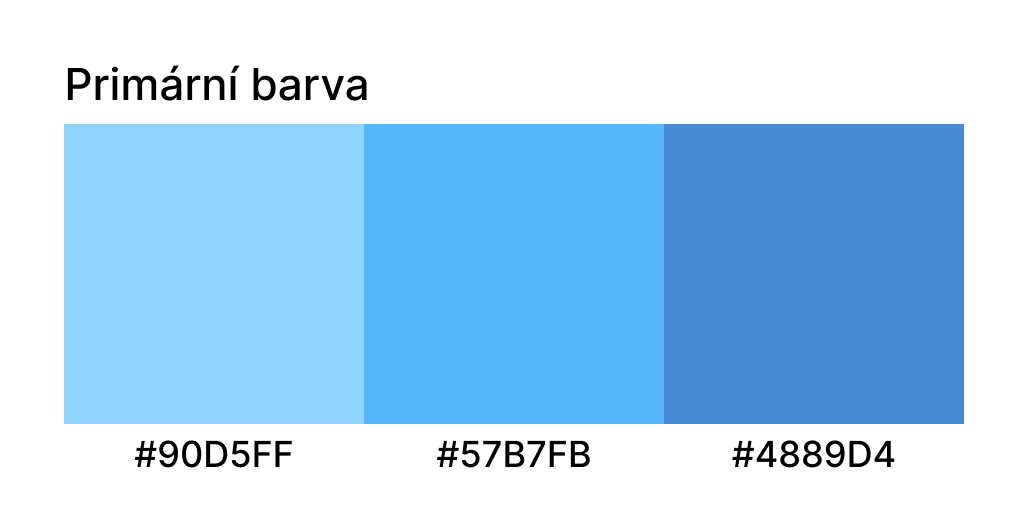
\includegraphics[width=\textwidth]{./images/Primary Color.png}
        \caption{Volba primární barvy}
        \label{fig:primary-color}
    \end{minipage}
\end{figure}

% Final
\subsubsection{Sekundární barva}

% Final
Material Design 2 umožňuje kromě primární barvy také definovat sekundární barvu, která slouží k doplnění primární barvy, vytvoření vizuálního kontrastu a zvýraznění určitých prvků rozhraní. Na rozdíl od primární barvy, která typicky reprezentuje samotnou značku aplikace a je v rozhraní přítomna na většině míst, je sekundární barva používána střídměji a pouze u některých prvků UI. Prakticky se tak využívá například na zvýraznění odkazů, v přepínačích, indikátorech stavů aplikace nebo v tzv. \textit{floating action buttons}. Přestože Material Design 2 definuje tuto sekundární barvu, její volba a použití jsou volitelné. \cite{MaterialDesignColorSystem}

% Final
Při volbě sekundární barvy jsem vycházel z principů teorie barev a ze standardně používaných barevných schémat, která definují rozložení barev na barevném kruhu \cite{FigmaWhatIsColorTheory}. Tato schémata slouží jako praktický nástroj pro posouzení, které barvy se vhodně doplňují tak, aby bylo možné je spolu využít například v uživatelském rozhraní. Na základě těchto schémat je tak možné zvolit sekundární barvu, která bude vhodně doplňovat primární barvu a vytvářet tak vizuálně příjemný vzhled uživatelského rozhraní. Při výběru sekundární barvy jsem volil z následujících schémat.

% Final
\paragraph{Monochromatické schéma} Monochromatické schéma využívá jeden odstín a jeho světlejší či tmavší varianty. V rozhraní obvykle působí klidně a kompaktně. Je také snadné na použití, protože designeři musí pracovat pouze s jedním hlavním odstínem. \cite{FigmaWhatIsColorTheory}

% Final
\paragraph{Analogické schéma} Analogické schéma kombinuje sousední barvy na barevném kruhu. Toto schéma je často možné pozorovat v přírodě, kde se podobné odstíny barev často vyskytují blízko sebe. Výsledkem bývá harmonický, méně kontrastní a přírodně vypadající vzhled. \cite{FigmaColorWheel}

% Final
\paragraph{Komplementární schéma} Komplementární schéma využívá dvojici protilehlých barev na barevném kruhu. Vytváří tak vysoký kontrast, což je přínosné pro uchycení a zaměření pozornosti uživatele na důležité prvky UI. Toto schéma tak umožňuje využití kombinace teplejších a chladnějších odstínů v UI. \cite{FigmaColorWheel}

% Final
\paragraph{Rozděleně komplementární schéma} Rozděleně komplementární schéma vychází z komplementární dvojice odstínů, ale místo přímého protikladu jsou využity dvě sousední barvy k doplňkové barvě. V praxi tak designeři mají možnost využít více barev a paleta tak může působit vyváženěji. \cite{FigmaColorWheel} \cite{FigmaWhatIsColorTheory}

% Final
\paragraph{Triadické schéma} Triadické schéma pracuje se třemi barvami rovnoměrně rozmístěnými na barevném kruhu do tvaru rovnostranného trojúhelníku. Toto schéma může působit živěji a dynamičtěji, nicméně stále je třeba určit, která ze tří barev bude v UI dominantní a které barvy budou používány střídměji. \cite{FigmaColorWheel} 

% Final
\paragraph{Tetradické schéma} Tetradické schéma využívá čtyři barvy, které tvoří na barevném kruhu obdélník, často ve formě dvou komplementárních dvojic. Toto schéma nabízí široké možnosti kombinací, avšak jeho použití v designu UI může být náročné, zejména kvůli udržení konzistence ve využití jednotlivých barev. \cite{FigmaColorWheel}

% Final
\paragraph{Čtvercové schéma} Čtvercové schéma využívá, stejně jako předchozí tetradické schéma, čtyři barvy rozmístěné na barevném kruhu. V tomto schématu jsou ovšem barvy rozmístěny rovnoměrně do tvaru čtverce. Podobně jako tetradické schéma poskytuje čtvercové schéma širší možnosti využití jednotlivých barev, nicméně zvyšuje riziko vizuální roztříštěnosti, pokud nejsou stanovena a dodržována jasná pravidla pro použití jednotlivých barev. Oproti tetradickému schématu umožňuje čtvercové schéma sestavit vyrovnanější vzhled ve srovnání s vysokým kontrastem, který tetradické schéma může vytvářet. \cite{FigmaColorWheel}

% Final
V rámci výběru sekundární barvy jsem se rozhodl využít monochromatické schéma, tedy pracovat primárně s jedním odstínem modré a jeho variantami, a samostatnou sekundární barvu pro rozhraní nedefinovat. Toto rozhodnutí přímo plyne ze stanovených zásad minimalismu a důvěryhodnosti. Díky omezení počtu barev by tak mělo uživatelské rozhraní působit minimalističtěji a mělo by být snazší dodržet konzistentní využití barev napříč návrhem a aplikací. Zároveň, jelikož jsem jako primární barvu zvolil světle modrou, by mělo výsledné rozhraní působit klidným a méně rušivým dojmem \cite{FigmaLightBlue}. To bude podstatné zejména při samotném učení, kdy je uživatel vystaven vyšší kognitivní zátěži a příliš agresivní barvy by pro něj mohly být rozptylující.

% Final
Přestože jsem se rozhodl zvolit monochromatické schéma, a využívat tak hlavně primární barvu, bude aplikace obsahovat řadu dalších barev, které budou používány například pro indikaci stavů v aplikaci. Příkladem toho jsou indikace správných a špatných odpovědí uživatele při učení. Těmto barvám se budu věnovat v následujících sekcích.

% Final
\subsubsection{Stavové barvy}

% Final
Kromě zvolení primární a sekundární barvy je třeba také zvolit barvy pro indikaci různých stavů, které mohou v aplikaci nastat. Tyto barvy budou například použity pro indikaci správných a špatných odpovědí uživatele, nebo pro indikaci chyb a varování v aplikaci. Jako základní odstíny jsem zvolil zelenou pro indikaci úspěšných stavů, oranžovou pro indikaci varování a červenou pro indikaci chyb. Jelikož budou tyto barvy často používány při učení, rozhodl jsem se vybrat pastelové varianty těchto barev, aby působily méně agresivním dojmem. Podobně jako primární barva by tak měly působit klidně, příjemně a neměly by příliš rozptylovat uživatele při učení.

% Final
Podobně jako u primární barvy, umožňuje Material Design 2 definovat hlavní variantu \texttt{main}, světlou variantu \texttt{light} a tmavou variantu \texttt{dark} pro každou barvu. Dále knihovna Material UI umožňuje definovat také odpovídající barvu textu \texttt{contrastText} \cite{MUIPalette}, která je dostatečně kontrastní vůči dané barvě a dodržuje tak standard přístupnosti \textit{Web Content Accessibility Guidelines 2.2}, dále WCAG 2.2 \cite{WCAG22}. Pro každý stav jsem tak vybral varianty barev, jejichž ukázku lze nalézt na obrázku \ref{fig:status-colors}. 

% Final
\begin{figure}[!ht]
    \centering
    \begin{minipage}{0.6\textwidth}
        \centering
        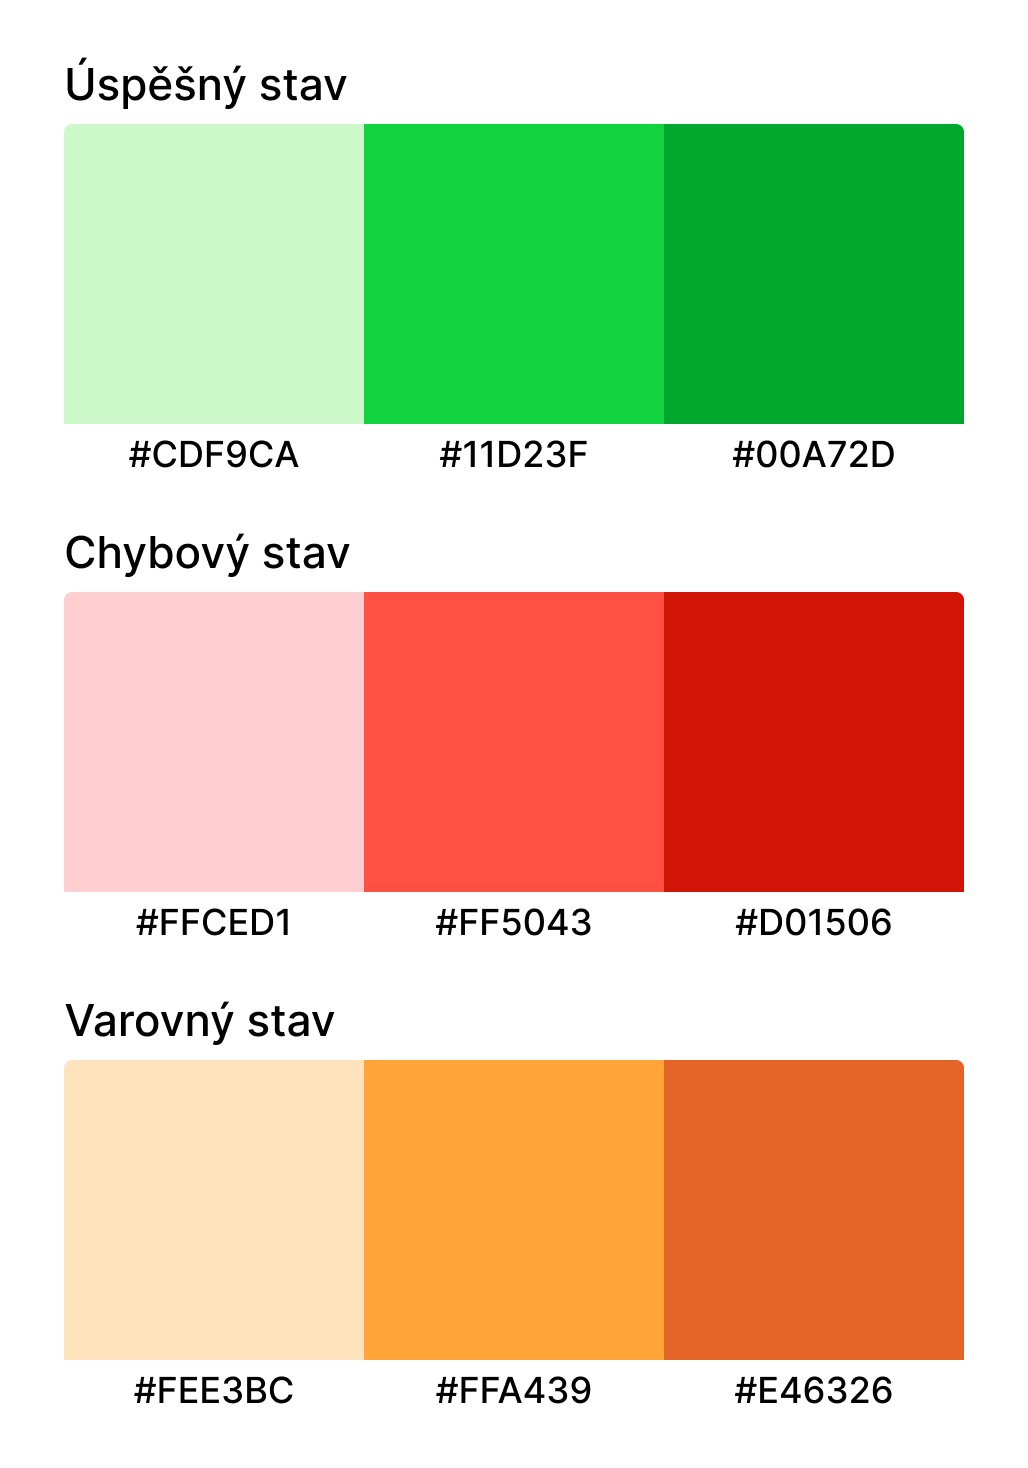
\includegraphics[width=\textwidth]{./images/Status Colors.png}
        \caption{Volba barev pro indikaci stavů}
        \label{fig:status-colors}
    \end{minipage}
\end{figure}

% Final
Podobně jako u primární barvy jsem pro volbu jednotlivých variant využil nástroj Material palette generator.

% Final
\subsubsection{Barvy pozadí}

% Final
Jako barvu pozadí \texttt{background} jsem se rozhodl využít výchozí barvu Material Design 2, tedy bílou barvu \texttt{\#FFFFFF}. Tato barva je používána zejména pro pozadí jednotlivých stránek. Jako barvu povrchů, neboli barvu pozadí některých komponentů, jsem dále zvolil světle šedou barvu \texttt{\#F3F3F3} označovanou jako \texttt{paper}, díky které bude možné komponenty lépe odlišit od pozadí stránek. Tyto barvy budou používány ve světlém režimu aplikace.

% Final
Ukázky barev pozadí a povrchů lze nalézt na obrázku \ref{fig:background-colors}.

% Final
\begin{figure}[!ht]
    \centering
    \begin{minipage}{0.5\textwidth}
        \centering
        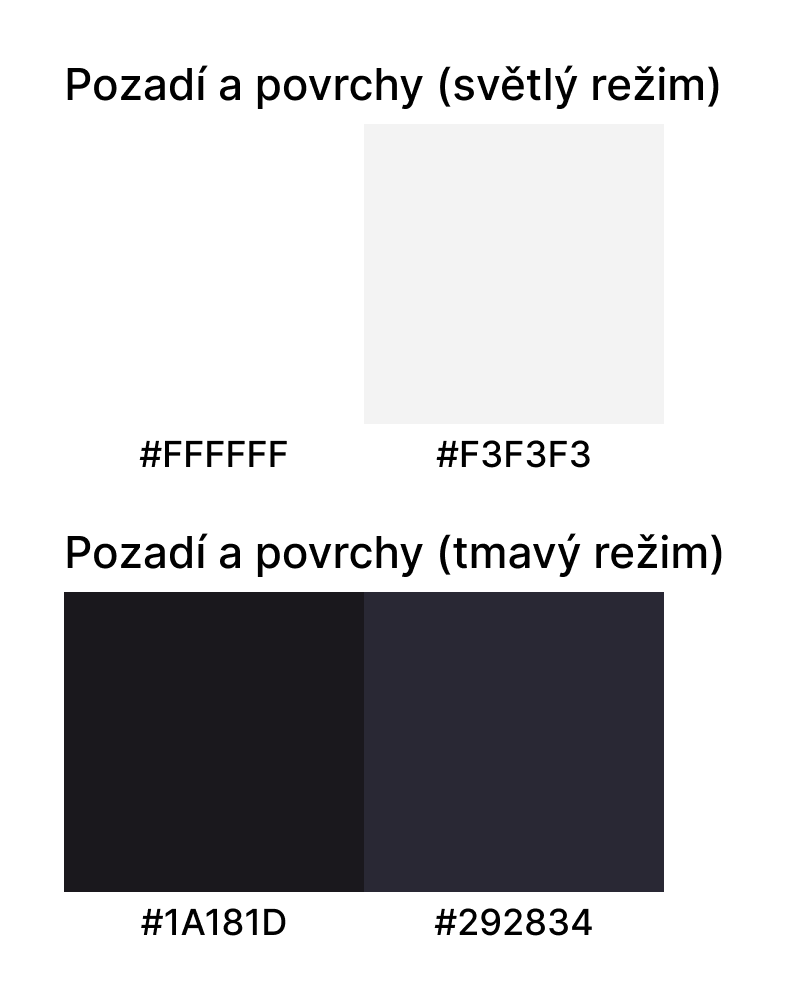
\includegraphics[width=\textwidth]{./images/Background Colors.png}
        \caption{Volba barev pozadí a povrchů}
        \label{fig:background-colors}
    \end{minipage}
\end{figure}

% Final
\subsubsection{Barvy textu}

% Final
Pro textové prvky jsem se rozhodl využít výchozí barvu Material Design 2, tedy černou barvu \texttt{\#000000}. Kromě této primární barvy textu knihovna Material UI ještě umožňuje definovat sekundární barvu textu, kterou je možné využít například pro odstavce a vytvořit tak silnější vizuální kontrast mezi nadpisy a běžným textem. Jako sekundární barvu jsem se tak rozhodl využít barvu \texttt{\#6f6f6f}, která je výrazně světlejší než černá barva, nicméně i pro běžný text stále splňuje kontrastní poměr mezi textem a barvami pozadí 4.5:1 dle AA standardu WCAG 2.2 \cite{WCAG22}.

% Final
\subsubsection{Tmavý režim}

% Final
Jedním z definovaných požadavků je dostupnost tmavého režimu aplikace. Pro vytvoření tmavého režimu je třeba jednotlivé barvy upravit tak, aby je bylo možné využívat na tmavých pozadích a aby stále odpovídaly standardu WCAG 2.2 \cite{WCAG22}. Při tvorbě tmavého režimu jsem postupoval dle doporučení oficiální dokumentace Material Design 2 \cite{MaterialDesign2DarkTheme}.

% Final
Jako první krok jsem se rozhodl zvolit samotné barvy pozadí a povrchů pro tmavý režim. Jako barvu pozadí jsem zvolil tmavě šedou barvu \texttt{\#1A181D} a jako barvu povrchů jsem dále zvolil lehce světlejší šedou barvu \texttt{\#292834}. Hlavním důvodem pro použití tmavě šedých barev, místo čistě černé barvy, je snaha dosáhnout nižšího kontrastu mezi světlým textem a tmavým pozadím. Text je pak lépe čitelný a méně namáhá oči uživatele. \cite{MaterialDesign2DarkTheme}

% Final
Po vybrání barvy pozadí je třeba přizpůsobit saturaci primární barvy, barvy stavů a barvy textu tak, aby byl dodržen kontrastní poměr 4.5:1 mezi textem a tmavým pozadím \cite{WCAG22}. Pro nalezení odpovídajících méně saturovaných barev jsem využil nástroj Colour contrast checker\footnote{Dostupné na: \href{https://colourcontrast.cc/}{https://colourcontrast.cc/}}, který mi umožnil vybrat k jednotlivým barvám jejich méně saturované varianty a zkontrolovat dodržení kontrastního poměru.

% Final
Nakonec jsem vybral barvy textu pro tmavý režim. Jako primární barvu textu jsem zvolil výchozí bílou barvu \texttt{\#FFFFFF} a jako sekundární barvu jsem zvolil \texttt{\#989898}. Obě barvy opět splňují požadovaný kontrastní poměr.

% Final
\subsection{Typografie}

% Final
V této sekci se zaměřím na volbu písma. Podobně jako u volby palety barev budu vycházet ze standardu Material Design 2 a budu volit vlastnosti písma v souladu se standardem přístupnosti WCAG 2.2 \cite{WCAG22}.

% Final
\subsubsection{Výběr písma}

% Final
Jako základní písmo jsem se rozhodl využít rodinu písem Inter\footnote{Dostupné na: \href{https://rsms.me/inter/}{https://rsms.me/inter/}}. Tato rodina písem byla publikována v roce 2017, zaměřuje se na moderní a čistý vzhled, podporuje přes 147 jazyků a je široce využívána napříč různými obory. Pro tuto rodinu písem jsem se rozhodl zejména z důvodu moderního a profesionálního vzhledu a její široké podpory a rozšířenosti. \cite{Inter}

% Final
Při volbě písma je možné dále využít tzv. párování fontů \cite[271-272]{Tidwell2020DesigningInterfaces}, při kterém se pro nadpisy využije jiná rodina písma, než pro běžný text. Díky tomu lze dosáhnout výraznějšího rozlišení mezi nadpisy a běžným textem a také zajímavějšího vzhledu rozhraní. Při tomto párování je ovšem třeba použít písma, která jsou od sebe dostatečně odlišná a využít tak například patková a bezpatková písma. Pro zachování minimalismu jsem se rozhodl toto párování nevyužít a použít tak rodinu písem Inter pro nadpisy i běžný text.

% Final
Dále, jelikož budou v aplikaci často využívány ukázky kódu, bylo potřeba zvolit písmo pro zobrazování kódu. Pro tento účel jsem se rozhodl využít rodinu písem JetBrains Mono\footnote{Dostupné na: \href{https://www.jetbrains.com/lp/mono/}{https://www.jetbrains.com/lp/mono/}}, která je speciálně navržena tak, aby byla dobře použitelná v editorech kódu a aby byl samotný kód dobře čitelný. \cite{JetBrainsMono}

% Final
\subsubsection{Hierarchie a škálování}

% Final
Po výběru rodiny písma je třeba dále zvolit typografickou škálu, která bude určovat velikosti jednotlivých textových prvků rozhraní, jako například velikosti nadpisů, podnadpisů a odstavců. Prvním krokem při volbě škály je zvolení základní velikosti písma, například 16 pixelů. Tato velikost reprezentuje velikost běžného textu v odstavcích. Následně se, na základě zvolené škály, toto číslo násobí daným poměrem, čímž se získají velikosti nadpisů, podnadpisů a dalších textových prvků.

% Final
Volba typografické škály tak určuje, jaký je rozdíl mezi velikostmi jednotlivých textových prvků. Tento rozdíl pak ovlivňuje, jak velký bude vizuální kontrast mezi jednotlivými prvky. Škály s vysokým kontrastem, jako například \textit{Golden ratio} s poměrem 1,618, jsou vhodné pro velké obrazovky \cite{TypographicScales}. Naopak škály s nízkým kontrastem, jako například \textit{Major Second} s poměrem 1,125, umožňují zobrazit větší množství textu na jedné stránce, jelikož jednotlivé textové prvky nezabírají tolik prostoru. Takové škály se často používají například na mobilních zařízeních, kde je prostor na obrazovce omezený.

% Final
Při volbě škály jsem nejprve použil oficiální nástroj pro generaci typografické škály dle standardu Material Design 2 \cite{MaterialDesign2TypeSystem}. Po aplikaci této škály při návrhu uživatelského rozhraní jsem ovšem došel k názoru, že tato škála vytváří příliš vysoký kontrast mezi textovými prvky. Velké nadpisy zabíraly příliš mnoho prostoru a byly při návrhu rozhraní pro tento typ aplikace takřka nepoužitelné. Nedostatek menších nadpisů tak neumožňoval dosáhnout detailnějšího odlišení jednotlivých sekcí a podsekcí v aplikaci, což značně znepřehledňovalo například stránky se cvičeními a vysvětlením látky. Došel jsem tak k závěru, že výchozí typografická škála Material Design 2 není pro tuto aplikaci vhodná.

% Final
Z tohoto důvodu jsem se rozhodl zvolit vlastní typografickou škálu, která bude vhodnější pro tento typ aplikace. Rozhodl jsem se vybrat dvě škály, jednu pro mobilní zařízení a jednu pro desktopová zařízení. Pro mobilní zařízení jsem se rozhodl využít škálu s nižším kontrastem \textit{Minor Third} s poměrem 1.200 a pro desktopová zařízení škálu \textit{Major Third} s poměrem 1,250. Díky těmto škálám tak bude možné plně využít všechny velikosti nadpisů a text tak bude lépe přizpůsoben velikostem jednotlivých zařízení. \cite{TypographicScales}

% Final
Pro generaci konkrétních velikostí písma jsem následně využil nástroj Typescale\footnote{Dostupné na: \href{https://typescale.com/}{https://typescale.com/}}. Při aplikaci vygenerované škály v návrhu rozhraní jsem následně dodržoval standardy Material Design 2, které se týkají vlastností jednotlivých textových prvků a definují například doporučené rozmezí velikostí písma.

% Final
\subsection{Ikony a ilustrace}

% Final
V rámci návrhu rozhraní je dále třeba zvolit vhodnou kolekci ikon a ilustrací. Pro vzhled ikon jsem se rozhodl využít kolekci Material Icons\footnote{Dostupné na: \href{https://fonts.google.com/icons}{https://fonts.google.com/icons}}. Pro návrh jsem se rozhodl využít zaoblenou variantu těchto ikon, aby rozhraní působilo hravějším a zábavnějším dojmem.

% Final
Jelikož bude aplikace obsahovat různé formy gamifikace a další motivační prvky, je třeba do návrhu zahrnout, kromě základních ikon, i různé ilustrace. Jako zdroj ilustrací jsem se rozhodl využít repozitář ilustrací publikovaných pod svobodnými licencemi SVG Repo\footnote{Dostupné na: \href{https://www.svgrepo.com/}{https://www.svgrepo.com/}}. Jednotlivé ilustrace jsem se pak snažil volit tak, aby měly vzájemně konzistentní styl.

% Final
\subsection{Animace a zvukové efekty}

% Final
V rámci návrhu jsem se dále rozhodl, v souladu s nefunkčními požadavky, navrhnout i animace a efekty, které by měly být při implementaci použity. Příslušné animace a efekty jsem vyznačil poznámkami u jednotlivých stránek v návrhu uživatelského rozhraní.

% Final
Mezi použité animace patří například animace přechodu mezi stránkami, animace zmáčknutí tlačítka, animace konfet při dokončení lekce, animace indikátoru pokroku při učení a další.

% Final
Kuriozitou při návrhu rozhraní bylo využití zvukových efektů. Zvukové efekty bývají ve webových aplikacích využívány velice zřídka, zejména kvůli tomu, že často nejsou pro interakci s uživatelem potřeba a zbytečně by uživatele rušily při práci s aplikací. V jistých případech mohou být ovšem zvukové efekty vhodné pro podpoření určitých emocí u uživatele a pro zvýšení intenzity požitku z vykonání určitých akcí. V této aplikaci tak budu využívat zvukové efekty například při samotném učení uživatele pro indikaci správných a špatných odpovědí nebo při úspěšném dokončení lekce. Jako zdroj zvukových efektů jsem se rozhodl využít soubor efektů Material Product Sounds\footnote{Dostupné na: \href{https://m2.material.io/design/sound/sound-resources.html}{https://m2.material.io/design/sound/sound-resources.html}}. Podobně jako u animací jsem vyznačil zvukové efekty v návrhu uživatelského rozhraní na místech, kde by měly být použity. \cite {MaterialDesign2ApplyingSounds}
